%!TEX root = Report.tex
\chapter{Results}\label{sec:results}

\subsection{Velocities}

First of all we see that the velocity in axial direction (Figure \ref{fig:v_x}) is significantly bigger as the ones in radial and tangential direction (Figures \ref{fig:v_r} and \ref{fig:v_theta} respectively). This is due to the fact that the fluid is only slightly deviated by the blades in radial and tangential directions. 

In Figure \ref{fig:v_x} we see how the velocity (in axial direction) is highest on the sides of the measurement area. In the middle, we see a decrease of velocity due to the stator blade. We see in both plots, how towards the inner tube and outer shell the velocity drops due to the wall-friction.\\



\begin{figure}[H]
\centering
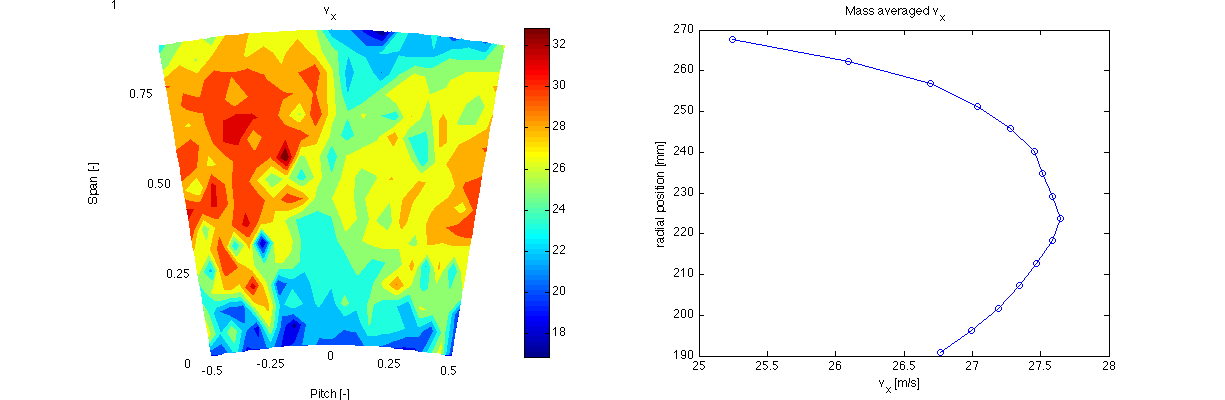
\includegraphics[trim = 110px 0px 80px 0px, clip = true,width=\textwidth]{pics/vx.png}
\caption{Measured Axial Velocity Over The Measuring Range And Mass Averaged Axial Velocity Over The Measured Pitch}
\label{fig:v_x}
\end{figure}
For a clearer analysis we plotted only the absolute value of $v_\theta$ in Figure \ref{fig:v_theta}, the direction of the velocity can be analysed in the angle section. In both plots we see the influence of the rotating inner tube on the fluid. As it is expected, there is a higher tangential velocity towards the axis due to the friction of the inner tube. The influence towards the outer wall is much lower. In the measurement area we see that the values are not constant throughout the pitch at the different radii. This comes from the influence of the stator blade.



\begin{figure}[H]
\centering
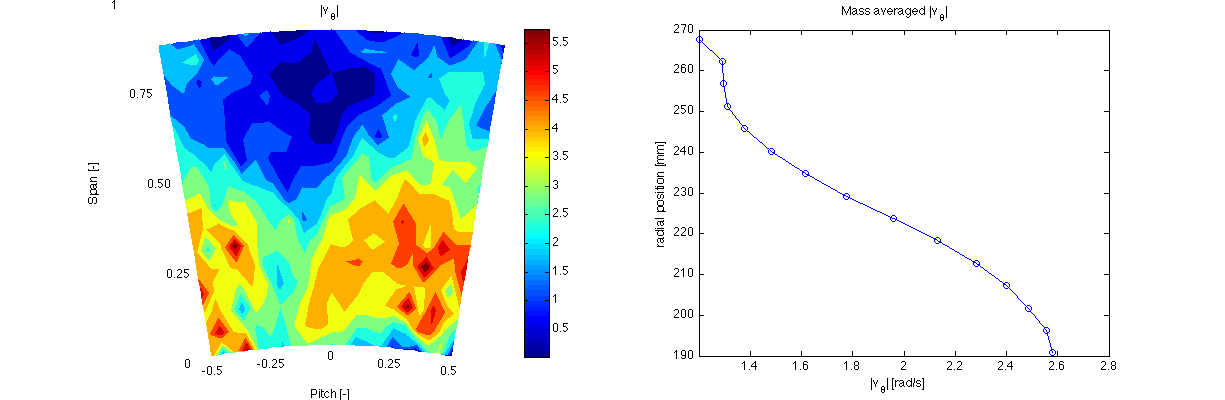
\includegraphics[trim = 110px 0px 80px 0px, clip = true,width=\textwidth]{pics/vtheta.png}
\caption{Measured Tangential Velocity Over The Measuring Range And Mass Averaged Tangential Velocity Over The Measured Pitch}
\label{fig:v_theta}
\end{figure}

In Figure \ref{fig:v_r} we see clearly an influence of the stator blade since the measurement area has a drop in velocity on the rght side. On the left side we a slow increase of velocity when moving from the inner tube to the outer wall, the mass averaged plot confirms this tendency. The cause for this phenomenon is the centrifugal force that drags the fluid to the outside. As the velocity of the blades is faster when the distance is greater from the rotation axis. Of course, the radial velocity should be zero when reaching the outer wall, but this deceleration of the fluid should happen between the gap of the measurement area and the wall itself.

\begin{figure}[H]
\centering
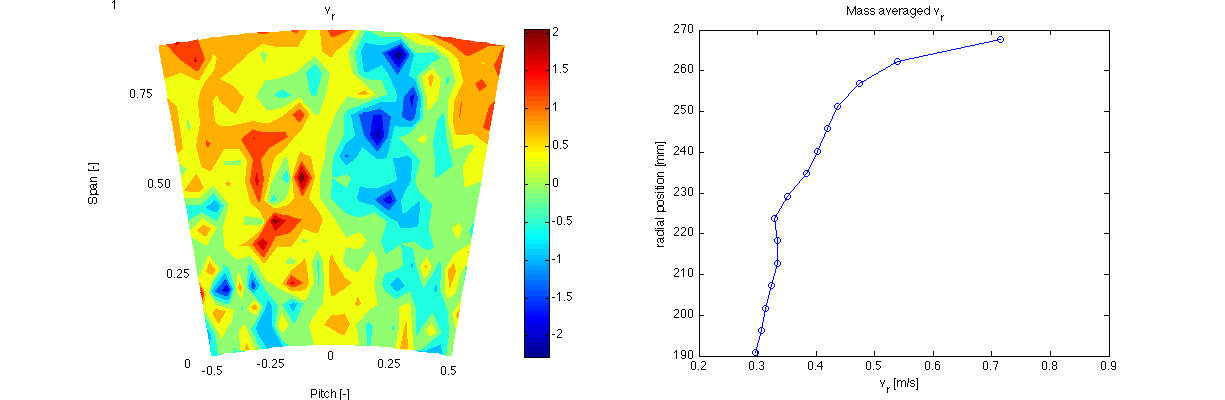
\includegraphics[trim = 110px 0px 80px 0px, clip = true,width=\textwidth]{pics/vr.png}
\caption{Measured Radial Over The Measuring Range And Mass Averaged Radial Velocity Over The Measured Pitch}
\label{fig:v_r}
\end{figure}

\subsection{Pressures}

In Figure $\ref{fig:ptot}$ the total pressure over the evaluated area and mass averaged is showed. The measured values at zero pitch angle show a decrease of pressure. This is due to the fact that the stator blade is in this position which causes friction and thus a loss of momentum. Near the walls the same effect takes place but in a higher degree, we conclude therefore that the friction is the highest in the area of the rotating axis).\\

\begin{figure}[H]
\centering
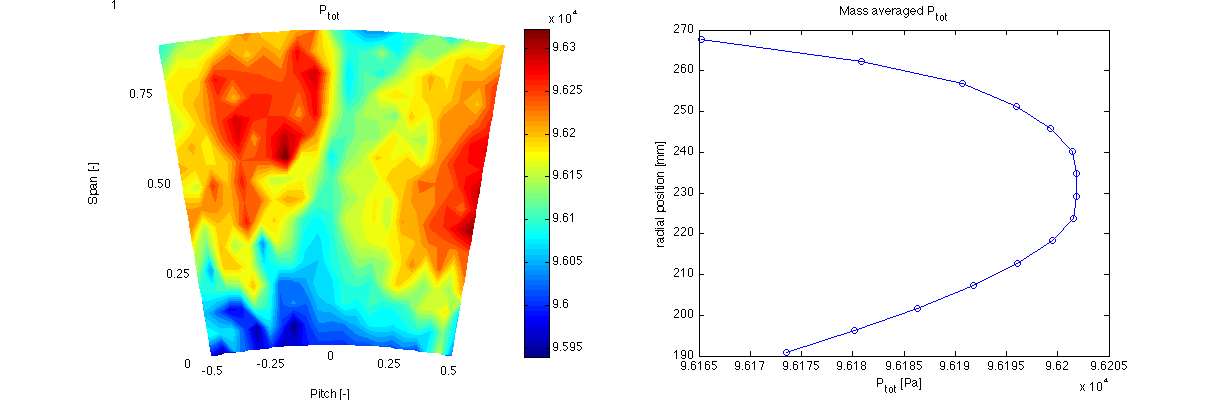
\includegraphics[trim = 110px 0px 80px 0px, clip = true,width=\textwidth]{pics/ptot.png}
\caption{Measured Total Pressure Over The Measuring Range And Mass Averaged Total Pressure Over The Measured Pitch}
\label{fig:ptot}
\end{figure}

In the mass averaged plot we see the maximum $p_{tot}$ towards the middle of the measured radii. In this area the friction is minimized due to the maximal distance to the turbine shell and rotation axis. 

\begin{figure}[H]
\centering
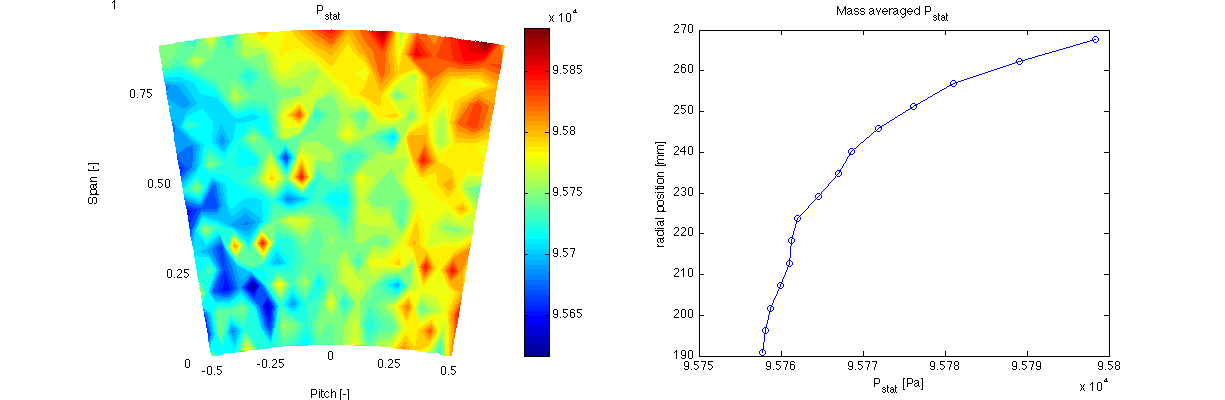
\includegraphics[trim = 110px 0px 80px 0px, clip = true,width=\textwidth]{pics/pstat.png}
\caption{Measured Static Pressure Over The Measuring Range And Mass Averaged Static Pressure Over The Measured Pitch}
\label{fig:pstat}
\end{figure}

To understand the results of the static pressure we have to work with the velocity of the fluid (\ref{fig:vtot}) as it is bounded to the static pressure $p_\text{stat}$ over the Bernoulli equation (Equation \ref{eq:bernoulli}). 

\begin{equation}
p_\text{tot} = p_\text{stat} + \rho \frac{v_\text{tot}^2}{2}
\label{eq:bernoulli}
\end{equation}
  
The results for $p_\text{stat}$ are showed in Figure $\ref{fig:pstat}$. In the measured area we cannot see an effect of the stator blade as clearly as in the previous figure. However we see a clear gradient of pressure over the pitch angle. We see a rise in static pressure on the upper right and a slight pressure drop on the left side due to the circulation of the fluid around the blade: The total velocity on the upper right side should therefore be lower and higher on the left side which matches with the measurements of Figure \ref{fig:vtot}

\begin{figure}[H]
\centering
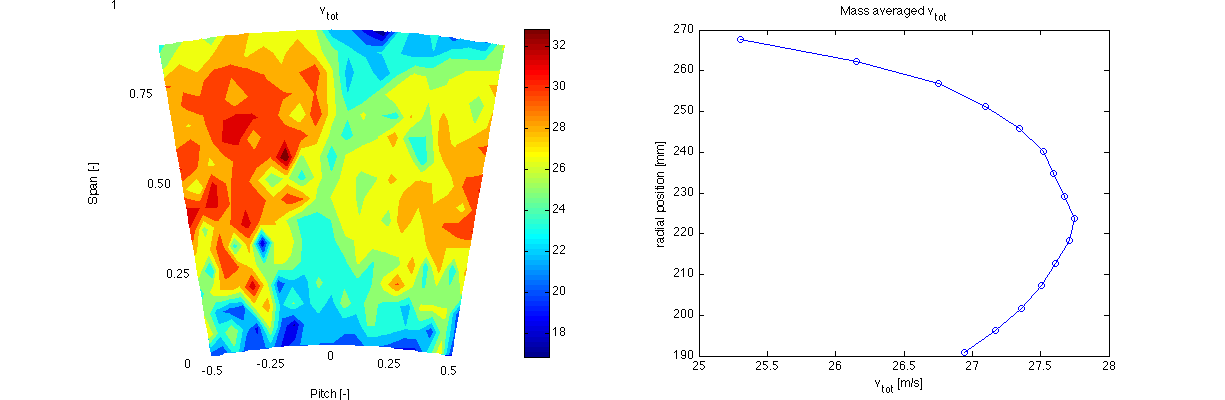
\includegraphics[trim = 110px 0px 80px 0px, clip = true,width=\textwidth]{pics/vtot.png}
\caption{Measured Total Velocity Over The Measuring Range And Mass Averaged Total Velocity Over The Measured Pitch}
\label{fig:vtot}
\end{figure}

By analysing the mass averaged plots we observe how the total velocity decreases towards the outer shell making an increase of static pressure in the same zone. Towards the inner tube, the velocity decreases again, this time not as much as towards the outer wall. The static pressure stays almost constant in that zone, which means that the loss of total pressure that we observe in Figure \ref{fig:ptot} comes almost entirely from the decrease of total velocity.

\subsection{Mach number}

From Equation \ref{eq:schallg} we can trace the correlation between $p_\text{stat}$ and $v_\text{tot}$.

\begin{equation}
Ma = \frac{v_\text{tot}}{c} = \frac{v_\text{tot}}{\sqrt{\gamma \frac{p_\text{stat}}{\rho}}}
\label{eq:schallg}
\end{equation}

 From our measurements we would expect a high $Ma$-number on the left side and a relatively low $Ma$-number on the upper right. This matches the measurements for $Ma$-number (Figure \ref{fig:mach} quite well. On the lower part we have the lowest $Ma$-number because of the low velocity and high static pressure.





\begin{figure}[H]
\centering
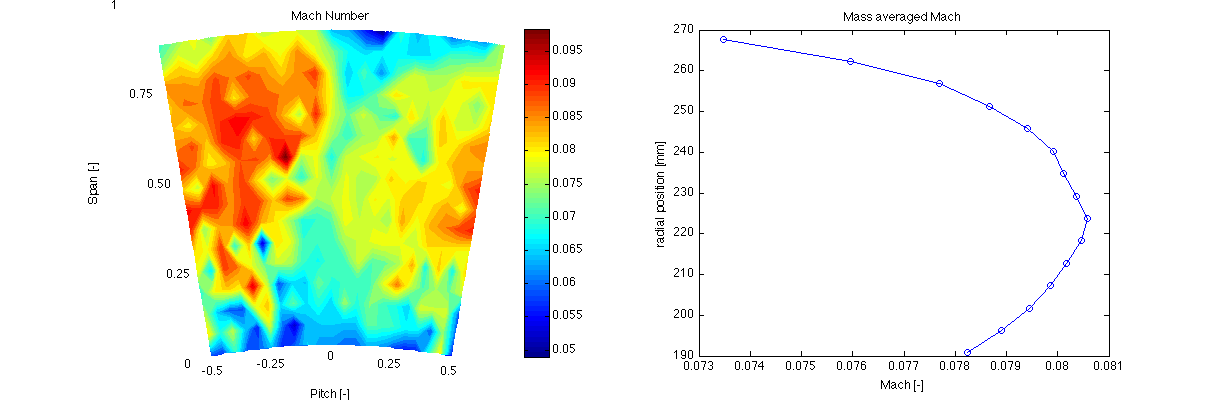
\includegraphics[trim = 110px 0px 80px 0px, clip = true,width=\textwidth]{pics/mach.png}
\caption{Measured Mach-number Over The Measuring Range And Mass Averaged Mach-number Over The Measured Pitch}
\label{fig:mach}
\end{figure}


Working analogously with Equation \ref{eq:schallg}, we see the correlations between the mass averaged plots of $p_\text{stat}$, $v_\text{tot}$ and $Ma$. In the lower part of the plots $p_\text{stat}$ behaves like a constant making the curve of $Ma$ similar to the one of $v_\text{tot}$. In the middle and upper part of the plots $v_\text{tot}$ decreases and $p_\text{tot}$ increases making the curve of $Ma$-number fall when approaching the wall. 

\subsection{Angles}

In the Figure \ref{fig:pitch}, the Pitch angle is plotted. A clear tendency is not visible. The pitch angle is only slightly higher on the left hand side. In the mass averaged plot, we can see that the pitch angle increases to the outer wall. This correlates with the radial velocity, that is increased when moving away from the rotational axis.
 
\begin{figure}[H]
\centering
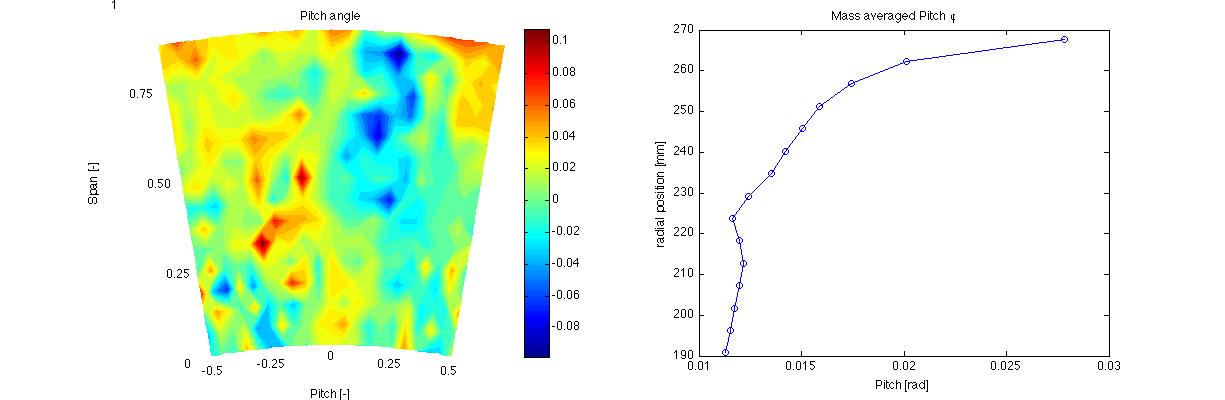
\includegraphics[trim = 110px 0px 80px 0px, clip = true,width=\textwidth]{pics/pitch.png}
\caption{Measured Pitch Angle Over The Measuring Range And Mass Averaged Pitch Angle Over The Measured Pitch}
\label{fig:pitch}
\end{figure}

Figure \ref{fig:yaw} shows the yaw angle. Near the rotational axis, the yaw angle is higher than near the outer walls. In this area the fluid is more deflected, due to the shape of the blade, just as expected. In the mass averaged plot, this becomes even more visible. In addition, we can observe a correlation with the tangential velocity,  which has its maximum near the rotational axis.

\begin{figure}[H]
\centering
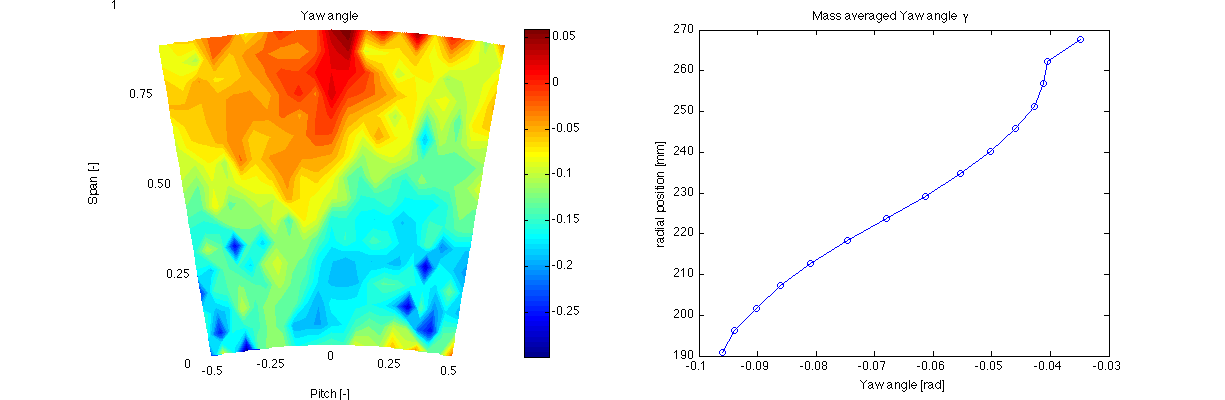
\includegraphics[trim = 110px 0px 80px 0px, clip = true,width=\textwidth]{pics/yaw.png}
\caption{Measured Yaw Angle Over The Measuring Range And Mass Averaged Yaw Angle Over The Measured Pitch}
\label{fig:yaw}
\end{figure}

\subsection{Velocity Triangles}

\begin{figure}[H]
\centering
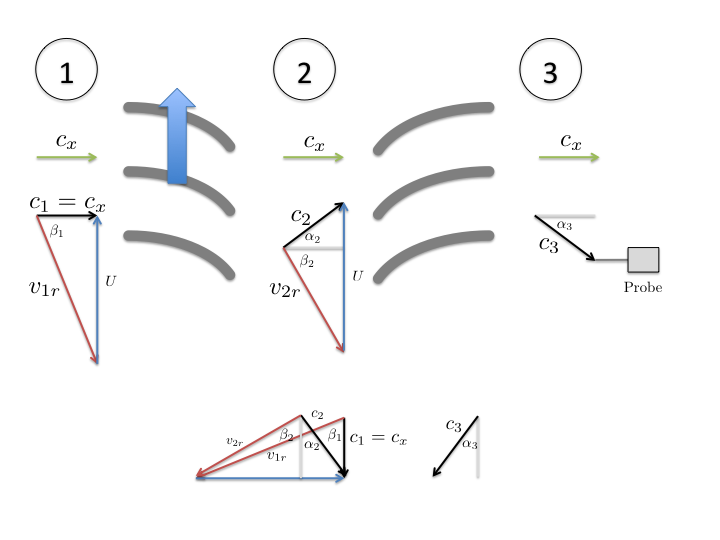
\includegraphics[width=\textwidth]{dreiecke.png}
\caption{Velocity Scheme Of A Compressor And Velocity Triangles}
\label{fig:dreiecke}
\end{figure}

In the Table \ref{tab:t1} we see can compare the different yaw angles to the actual blade angles at each height of the blade. We see that the fluid deviation decreases towards the inner tube.

\begin{table}[H]
\centering
    \begin{tabular}{|l|c|c|}
        \hline
        Span & Yaw angle (measured) [$^\circ$] & Yaw angle (blade) [$^\circ$] \\ \hline
        90\%  & -2.009                   & 9                     \\ 
        70\%  & -2.527                   & 8                     \\ 
        50\%  & -3.466                   & 6                     \\ 
        30\%  & -4.723                   & 4                     \\ 
        10\%  & -5.466                   & -0.5                  \\
        \hline
    \end{tabular}
\caption{Measured Yaw Angle And Stator Outlet Blade Angle Over The Measured Heights)}
\label{tab:t1}
\end{table}

To calculate the velocity triangles we worked consistently with the scheme shown in Figure \ref{fig:dreiecke}. We assumed an optimal flow and no incidence angle ($\alpha_1$) in the rotor inlet. The outlet angle of the stator ($\alpha_3$) is assumed to be the measured yaw angle. 

\begin{table}[H]
\centering
    \begin{tabular}{|l|l|l|l|l|l|l|l|l|l|}
        \hline
        Span & $U$ [$\frac{m}{s}$] & $c_3$ [$\frac{m}{s}$]  & $c_2$ [$\frac{m}{s}$] & $c_1$ [$\frac{m}{s}$] & $v_{2r}$ [$\frac{m}{s}$] & $v_{1r}$ [$\frac{m}{s}$] & $v_{x}$ [$\frac{m}{s}$] & $v_{r}$ [$\frac{m}{s}$] & $v_{\theta}$ [$\frac{m}{s}$] \\ \hline
        90\%  & 140.115                   & 25.281  & 31.635 & 25.265      & 123.684  & 142.375 &  25.265& 0.710 & -0.910    \\ 
        70\%  & 130.271                   & 27.146  & 35.180 & 27.146      & 111.257  & 133.070  & 27.146 & 0.429 & -1.199 \\ 
        50\%  & 120.428                   & 27.576  & 36.820 & 27.576      & 99.911   & 123.545  & 27.576 & 0.355 & -1.673 \\ 
        30\%  & 110.584                   & 27.433  & 38.797 & 27.433      & 87.559   & 113.936  & 27.576 & 0.331 & -2.255 \\ 
        10\%  & 100.740                & 26.8371 & 42.645 & 26.837      & 72.732   & 104.254  & 26.837 & 0.300 & -2.524 \\
        \hline
    \end{tabular}
\caption{Calculated Velocities Of The Velocity Triangles}
\label{tab:t2}
\end{table}

With help of basic trigonometric relations we were able to calculate the rest of the angles and velocities including the inlet and outlet angles of the rotor ($\beta_1$ and $\beta_2$). The results are listed in Tables \ref{tab:t2} and \ref{tab:t3}. 

\begin{table}[H]
\centering
    \begin{tabular}{|l|l|l|l|l|l|}
        \hline
        Span & $\alpha_3$ [$^\circ$] & $\alpha_2$ [$^\circ$] & $\beta_2$ [$^\circ$] & $\alpha_1$ [$^\circ$] & $\beta_1$ [$^\circ$] \\ \hline
        90\%  & -2.009                & 37.000                & 78.213               & 0                     & 79.778               \\ 
        70\%  & -2.527                & 39.500                & 75.878               & 0                     & 78.229               \\ 
        50\%  & -3.466                & 41.500                & 73.978               & 0                     & 77.102               \\ 
        30\%  & -4.723                & 45.000                & 71.741               & 0                     & 76.068               \\ 
        10\%  & -5.466                & 51.000                & 68.347               & 0                     & 75.083               \\
        \hline
    \end{tabular}
\caption{Calculated Angles Of The Velocity Triangles}
\label{tab:t3}
\end{table}

